% Journal:
%   Journal of Ambient Intelligence and Smart Environments (JAISE), IOS Press
%   Web Intelligence and Agent Systems: An International Journal (wias)
%   Semantic Web: Interoperability, Usability, Applicability (SW)
% Latex 2e
% Test file iosart2c.tex

%[seceqn,secfloat,secthm,crcready]

% options: wias, jaise, sw
\documentclass{iosart2c}

\usepackage[T1]{fontenc}
\usepackage{times}%
\usepackage{listings}
\usepackage{tabularx}
\usepackage{algorithm}
\usepackage{pdflscape}
\usepackage{url}
\usepackage{natbib}% for bibliography sorting/compressing
%\usepackage{amsmath}
%\usepackage{endnotes}
\usepackage{graphics}
\usepackage{xcolor}
\usepackage{epsfig,color,subfigure}
%\usepackage{bibentry}

%%%%%%%%%%% Put your definitions here
\newcommand{\TODO}[1]{\textcolor{red}{\textbf{[TODO:#1]}}}
\newcommand{\maria}[1]{\textcolor{blue}{\textbf{[MARIA TO:#1]}}}
\newcommand{\py}[1]{\textcolor{olive}{\textbf{[PIERRE-YVES TO:#1]}}}
\newcommand{\ghis}[1]{\textcolor{brown}{\textbf{[GHIS TO:#1]}}}

% Language Definitions for Turtle
\definecolor{olivegreen}{rgb}{0.2,0.8,0.5}
\definecolor{grey}{rgb}{0.5,0.5,0.5}
\lstdefinelanguage{ttl}{
sensitive=true,
morecomment=[l][\color{brown}]{@},
morecomment=[l][\color{red}]{\#},
morestring=[b][\color{blue}]\",
}

%% language json
\colorlet{punct}{red!60!black}
\definecolor{background}{HTML}{EEEEEE}
\definecolor{delim}{RGB}{20,105,176}
\colorlet{numb}{magenta!60!black}

\lstdefinelanguage{json}{
    basicstyle=\normalfont\ttfamily,
    numbers=left,
    numberstyle=\scriptsize,
    stepnumber=1,
    numbersep=8pt,
    showstringspaces=false,
    breaklines=true,
    frame=lines,
    backgroundcolor=\color{background},
    literate=
     *{0}{{{\color{numb}0}}}{1}
      {1}{{{\color{numb}1}}}{1}
      {2}{{{\color{numb}2}}}{1}
      {3}{{{\color{numb}3}}}{1}
      {4}{{{\color{numb}4}}}{1}
      {5}{{{\color{numb}5}}}{1}
      {6}{{{\color{numb}6}}}{1}
      {7}{{{\color{numb}7}}}{1}
      {8}{{{\color{numb}8}}}{1}
      {9}{{{\color{numb}9}}}{1}
      {:}{{{\color{punct}{:}}}}{1}
      {,}{{{\color{punct}{,}}}}{1}
      {\{}{{{\color{delim}{\{}}}}{1}
      {\}}{{{\color{delim}{\}}}}}{1}
      {[}{{{\color{delim}{[}}}}{1}
      {]}{{{\color{delim}{]}}}}{1},
}
%%%%%%%%%%% End of definitions

\newcolumntype{d}[1]{D{.}{.}{#1}}


\firstpage{1} \lastpage{5} \volume{1} \pubyear{2014}


\begin{document}

\begin{frontmatter}                        % The preamble begins here.

%
%\pretitle{Pretitle}
\title{LOV: A gateway to reusable semantic vocabularies on the Web}
%\title{LOV: An Ontology-based search engine for the Web}
%\thanks{Footnote in title.}}

\runningtitle{LOV: A gateway to reusable semantic vocabularies on the Web}
%\subtitle{Subtitle}

\review{Name Surname, University, Country}{Name Surname, University, Country}{Name Surname, University, Country}


\author[A]{\fnms{Pierre-Yves} \snm{Vandenbussche}  \thanks{Thanks to Am\'elie Gyrard and Thomas Francart for their reviews on vocabularies}},
\author[B]{\fnms{Ghislain A.} \snm{Atemezing}\thanks{Corresponding author. E-mail: auguste.atemezing@eurecom.fr}},
\author[C]{\fnms{Mar\'ia} \snm{Poveda-Villal\'on}}
and
\author[D]{\fnms{Bernard} \snm{Vatant}}
\runningauthor{Pierre-Yves V. et al.}
\address[A]{Fujitsu (Ireland) Limited, Swords, Co. Dublin, Ireland\\
E-mail: pierre-yves.vandenbussche@ie.fujitsu.com}
\address[B]{Multimedia Communication Department, EURECOM, Campus SophiaTech
450, route des Chappes, 06410 Biot, France\\
E-mail: auguste.atemezing@eurecom.fr}
\address[C]{Ontology Engineering Group (OEG), 
Universidad Polit\'ecnica de Madrid, Madrid, Spain\\
E-mail: mpoveda@fi.upm.es}
\address[D]{Mondeca, 35 boulevard de Strasbourg, 75010 Paris, France
\\
E-mail: bernard.vatant@mondeca.com}


\begin{abstract}
\textcolor{red}{The abstract should be clear, descriptive, self-explanatory and no longer than 200 words. It should also
be suitable for publication in abstracting services. Do not include references or formulae in the abstract.}
\end{abstract}

\begin{keyword}
LOV\sep Linked Open Vocabulary\sep Ontology search\sep Linked Data
%\sep keyword five
\end{keyword}

\end{frontmatter}


\section{Introduction}
Started in March 2011, in the framework of the DataLift research project \cite{scharffe_2012} hosted by the Open Knowledge Foundation, the Linked Open Vocabularies (LOV) initiative is now standing as an innovative observatory of the semantic vocabularies\footnote{In this paper, ``semantic vocabulary'', ``vocabulary'' and ``ontology'' terms all refer to a collection of classes and properties expressed in W3C RDF, RDFS, OWL languages. A vocabulary is used to describe linked data on the Web.} ecosystem. It gathers and makes visible indicators not yet harvested before, such as interconnection between vocabularies, versioning history, maintenance policy and past and current referent (individual or organization) if any. The number of vocabularies indexed by LOV is constantly growing (469 as of December 2014) thanks to a community effort. It is the only catalog, to the best of our knowledge, that provide all types of search criteria (metadata search, within/across ontologies search), APIs, comprehensive dump file and a SPARQL endpoint access. According to the categories of ontology libraries defined in~\cite{AquinJoWS12}, LOV falls under the category of \textit{``curated ontology directory''}  and \textit{``application platform''}.

The development of LOV has highlighted a number of interesting research challenges such as \textit{``What are the solutions for long-term vocabulary preservation on the Web?"}\cite{Baker2013HLT}. This is a particularly important problem in a distributed and uncontrolled environment where any individual can create and publish a vocabulary that can then be reused by external publishers, creating a dependency on its availability to get access to the semantic. \textit{``How to facilitate vocabulary search and reuse"}\cite{butt2014, poveda2012landscape}. To be used by a broader community, the reuse and design of vocabularies has to be facilitated by intuitive tools and methods.  \textit{``How can we harmonise the various curated vocabulary catalogues on the Web to ease their adoption?"}\cite{wasabi13}. One of the barrier to Semantic Web adoption is the confusion in understanding and find an appropriate vocabulary.

The system report is structured as follows: In the next section, we describe the LOV architecture and the type of information we capture about vocabularies. This is followed by the main functionalities offered by LOV along with some usage analysis. In section \ref{sec:dataPubOntoEngine}, we explicate how LOV is used to support Data publication and Ontology Engineering process. Subsequently, we provide an overview of some applications and research projects based and motivated by LOV (Section \ref{sec:lovecosystem}). In Section \ref{sec:related}, we report on related work and conclude in section \ref{sec:conclusion}.


\section{A catalogue of vocabularies}
\label{sec:metadata}
A vocabulary to be accepted and inserted into LOV, a minimal metadata information is required in the vocabulary. Those metadata should be described reusing existing meta-vocabularies, such Dublin core, lexvo\footnote{\url{http://lexvo.org/ontology#}} and provenance vocabulary.
Three levels of metadata are present in any vocabulary in LOV:
\begin{itemize}
\item Metadata associated to the vocabulary: this information is embed in within the vocabulary to provide context, and useful data about the vocabulary. Four minimal metadata is asked to the publisher of a vocabulary to be LOV-able: title, description, dereferencable URI. The bot spots more information 

\item Inlinks vocabularies, using links to a given vocabulary

\item Outlinks vocubularies, that is vocabularies reused to create a given vocabulary.  
\end{itemize}

\begin{figure}[ht!b]
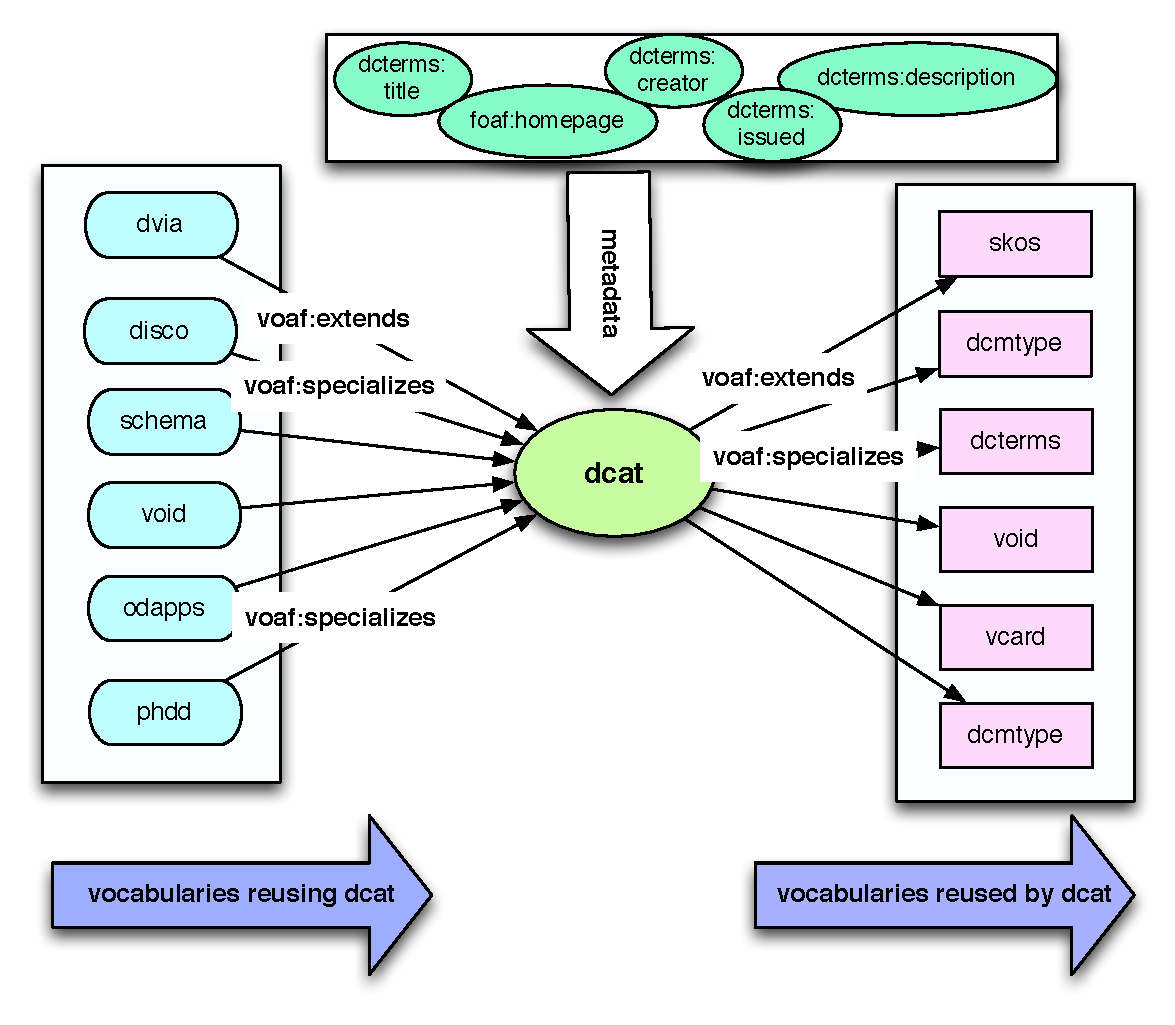
\includegraphics[scale=0.4]{dcat-relations.pdf}
\caption{Sample type of relations and metadata used in the DCAT vocabulary.}
\label{fig:dcat}
\end{figure}

Languages tag retrieved for each vocabulary is inserted into LOV database by using the \texttt{dcterms:language} property with the URI of the language in lexvo dataset using the ISO 639-3 code. For example, the URI associated to Japanese language is \url{http://www.lexvo.org/page/iso639-3/jpn}. Currently, 91.25\% (428 out of 469) of vocabularies use a language tag associated, with only 9 vocabularies with labels in a language different from English. Table \ref{tab:language} presents the number and percentage of the top five languages detected in LOV. This results suggest that publishers should make more effort to provide multilingual vocabularies on the Web,
 
 \begin{table}[h!tb]
\caption{Top five languages and percentage detected in LOV catalogue.}
\begin{tabular}{lcc}
\hline
\textbf{Language} & \textbf{Number} & \textbf{\%}  \\ \hline
English  & 419   &  97.89\%      \\
French & 42 & 9.81\% \\
Spanish & 28 & 6.54\%\\
German & 21 & 4.90\%\\
Italian & 20 & 4.67\%\\
\hline  
\end{tabular}
\label{tab:language}
\end{table}

\section{LOV functionalities}
\label{sec:about}

\py{ give some input here, and current figures}\\

LOV high-curated vocabularies are suitable for ontology search and reuse activities during the process of creating and publishing a vocabulary. Below are the relevant features of LOV achieving the aforementioned activities:

 \begin{description}
	\item [Domain filtering.] Each vocabulary is inserted into LOV according to its domain and/or scope. This information is guided by the scope of the vocabulary, such as City, Science, Library, Metadata, Media, etc. This feature helps in disambiguating the results of the querying service and to classify vocabularies.
	\item [Content aware Search.] If the searched term matches a \url{rdfs:label} it will have a higher score than if it matches \url{dcterms:comment}.
	\item [Links between vocabularies.] One of the key feature of LOV design is the explicit links between vocabularies,
	 \item [Scope of LOV.]The intended use is to promote and facilitate the reuse of vocabularies in the linked data ecosystem.
	 \item [Vocabulary curation.]The collection of the vocabularies is maintained by curators in charge of validating and inserting vocabularies in the LOV ecosystem, by taking care of the versions of the vocabulary and giving some reviews. The vocabulary is then automatically enriched with more information about the datasets using it, and relations to other vocabularies.
 \end{description}

%\todo{reference the image of vocabs evolution in LOV}

\begin{figure}[h!tb]
\centering
  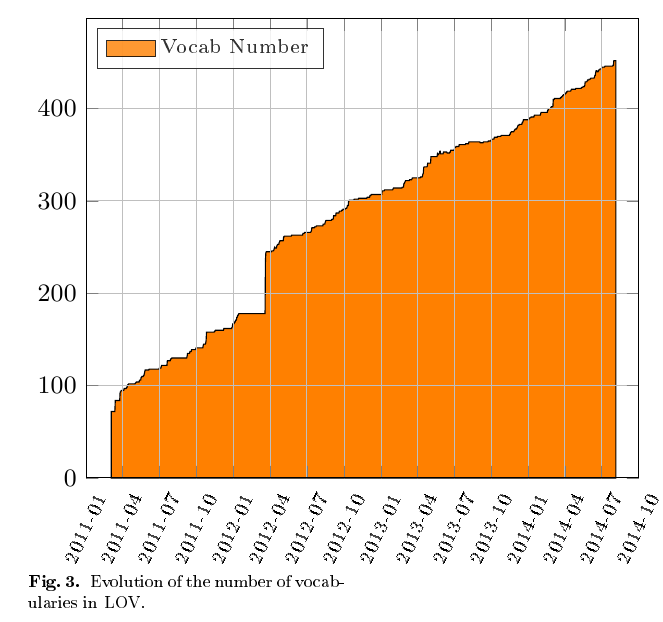
\includegraphics[width=\linewidth]{LOVEvol.png}
  \caption{Graph evolution of vocabularies inserted into LOV from 2011 to 2014.}
  \label{fig:translations}
\end{figure}

\subsection{LOV as an ontology search engine}
\label{sec:ontoSearch}
Users or agents use keywords to search properties or classes within vocabularies in the LOV catalogue. The log\footnote{\url{http://lov.okfn.org/dataset/lov/stats/searchLog.csv}} of search terms between 2012/01/06 and 2014/12/09 presents a total of 54,657 terms, with 36,019 (65.90\%) duplicate terms and 18,643 unique terms (34.10\%). Figure \ref{fig:searchterms} depicts the number of terms in the log grouped by year. From 2012 to 2013, there have been an increase of more than 50\% of terms for searching vocabularies in LOV. Searching terms are mostly single words (e.g., currency). However, terms can be composite of two words (e.g., ``family tree''), three words (e.g., ``semantic sensor network'') or an URI (e.g., ``http://www.aktors.org/ontology/portal''). Table \ref{tab:patterns} shows details for the use of URIs, two words and at least three words for unique values in the LOV searching log.


\begin{table}[h!tb]
\caption{Patterns used other than one term in searching vocabularies in LOV.}
\begin{tabular}{lcccc}
\hline
\textbf{Pattern} & \textbf{2012} & \textbf{2013} & \textbf{2014} & \textbf{Total} \\ \hline
\textit{URI}  & 38   &  54  & 63  &  155      \\
$t_{1}$ $t_{2}$ & 200 & 480 & 466 & 1146 \\
($t_{1}$ $t_{2}$ $t_{3}$)* & 93 & 233 & 249 & 575\\
\hline  

\end{tabular}
\label{tab:patterns }
\end{table}

\begin{figure}[!htbp]
\centering{
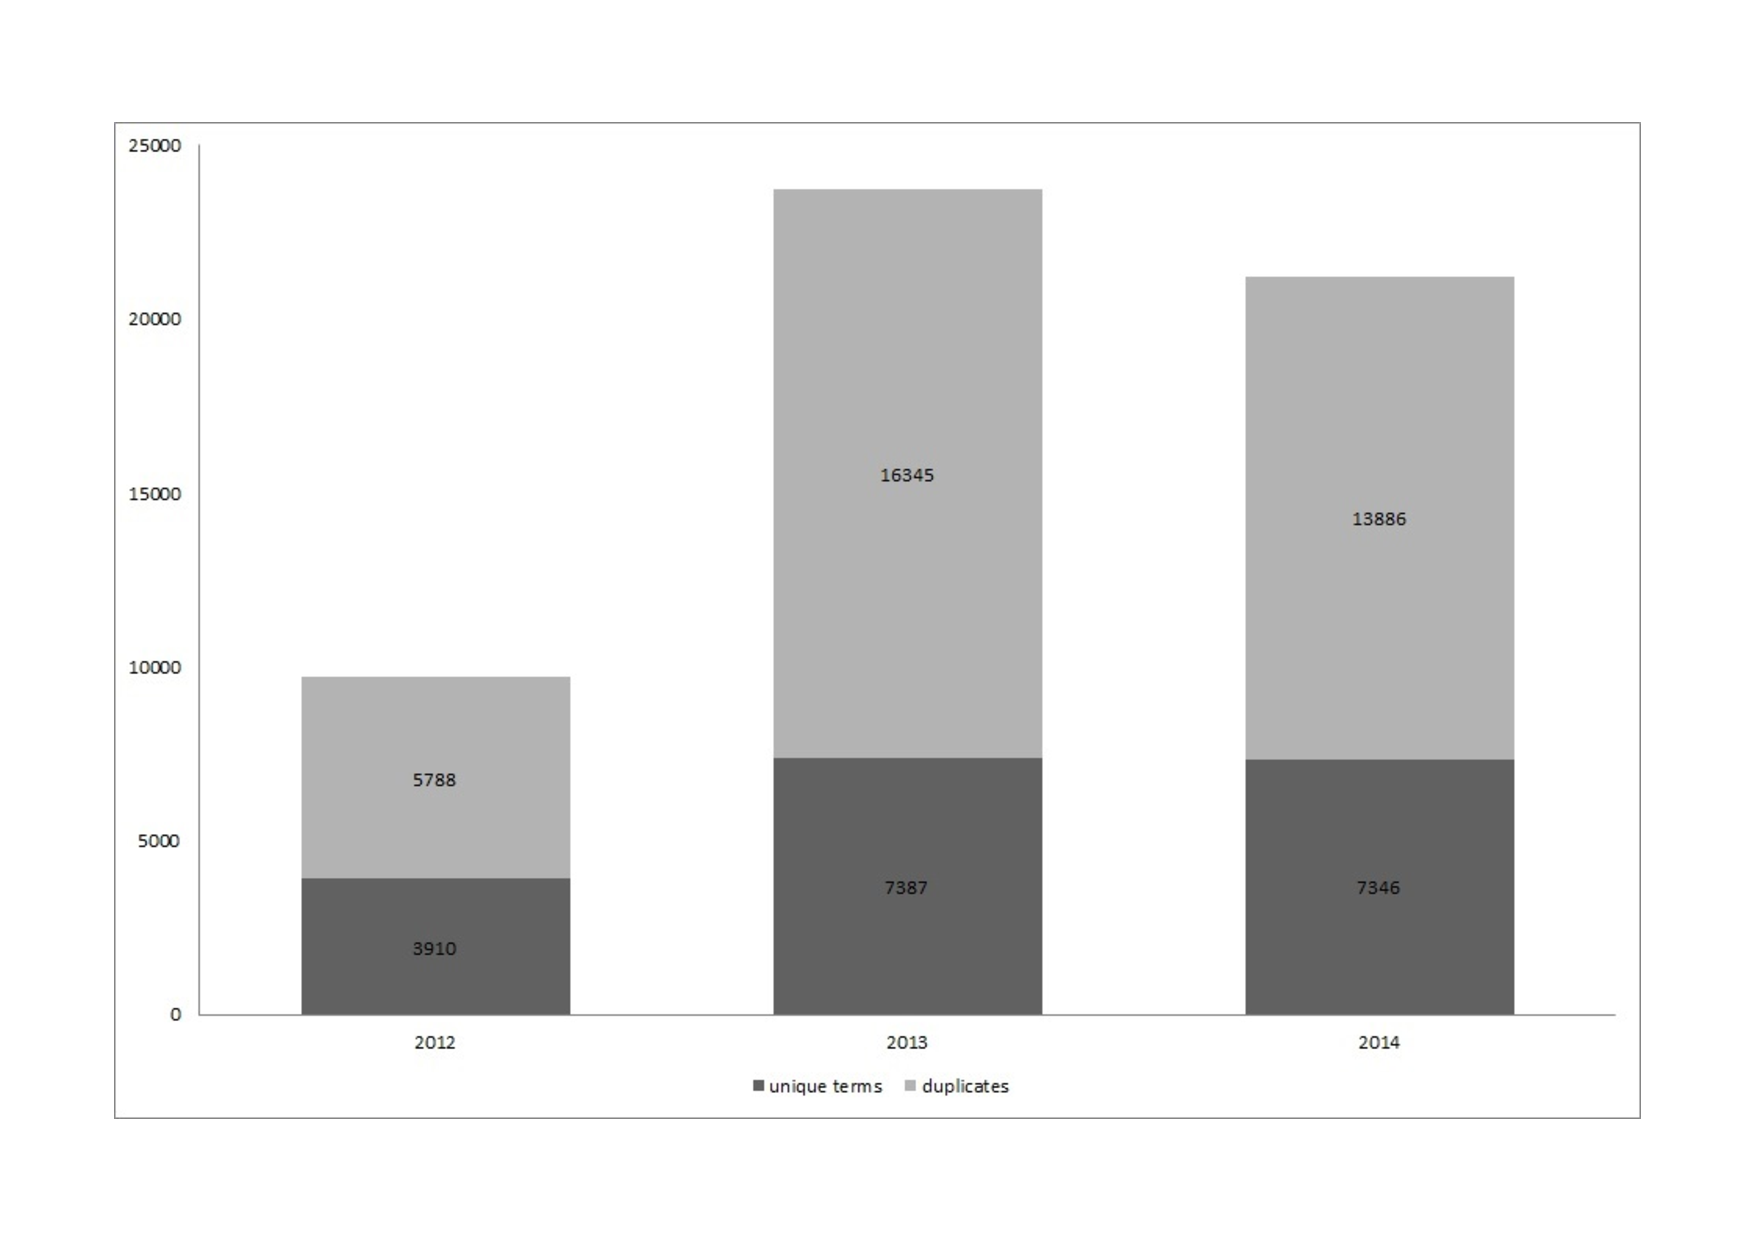
\includegraphics[scale=.28]{chart_searchterms.pdf}
\caption{Unique and duplicate terms searched by agents/users according to LOV log in the period between 2012/01/06 until 2014/12/09.}
\label{fig:searchterms}
}
\end{figure}


\section{LOV as a support for Data Publication and Ontology Engineering}
\label{sec:dataPubOntoEngine}

\subsection{Life-cycle of a vocabulary in LOV}
\label{sec:lifecyle}

\TODO{ ADD some text here }\\
Review --insertion --publication --archive version --Daily checking --\\

\ghis{ add a figure of tracking the vocabulary evolution}
\paragraph{Criteria to remove a vocabulary} 
When it is orphan, no metadata, no labels. 


\subsection{Building ontologies with LOV}
\label{sec:builOnto}

The NeOn Methodology is a scenario-based methodology that supports the collaborative aspects of ontology development and reuse, as well as the dynamic evolution of ontology networks in distributed environments. The key assets of the NeOn Methodology are \cite{MC10}:
\begin{itemize}
 \item  A set of nine scenarios for building ontologies and ontology networks, emphasizing the reuse of ontological and non-ontological resources, the re-engineering and merging, and taking into account collaboration and dynamism.
 \item The NeOn Glossary of Processes and Activities, which identifies and defines the processes and activities carried out when ontology networks are collaboratively built by teams.
 \item Methodological guidelines for different processes and activities of the ontology network development process, such as the reuse and re-engineering of ontological and non-ontological resources, the ontology requirements specification, the ontology localization, the scheduling, etc.
\end{itemize}


LOV is a catalog and API that can fits well within the Neon methodology for building vocabularies and ontologies. Based on the Neon Methodology's glossary of activities for building ontologies, LOV is relevant in four activities:


\begin{description}

 \item [Ontology Search.] Main LOV's feature is the search of vocabulary terms. These vocabularies are categorized within LOV according to the domain they address. In this way, LOV contributes to ontology search by means of (a) keyword search and (b) domain browsing.
 \item [Ontology Assessment.] LOV provides a score for each term retrieved by a keyword search. This score can be used during the assessment stage and includes a unique term statistical feature\footnote{\url{http://lov.okfn.org/dataset/lov/stats/}} which provides for each term registered in LOV the following information: (a) ``LOV distribution'' that represents the number of vocabularies in LOV that refer to a particular element; (b) ``LOV popularity'' that shows the number of other vocabulary elements that refers to a particular one; and (c) ``LOD distribution'' that refers to the number of datasets in LOD which use a particular vocabulary; and (d) ``LOD popularity'' that refers to the number of vocabulary element occurrences in the LOD.
 \item [Ontology Mapping.] In LOV, vocabularies rely on each other in seven different ways. These relationships are explicitly stated using VOAF vocabulary. This data could be useful to find alignments between ontologies, for example one user might be interested in finding equivalent classes for a given class or all the equivalent classes among two ontologies. Listing \ref{list:alignment} shows the retrieved data when asking for all the equivalent classes and properties between the vocabularies foaf and dcterms by means of the related VOAF query\footnote{\url{http://goo.gl/sTIGQ6}. Prefixes are omitted for readability purpose. The reader can find the correct namespace for a prefix in LOV.}:
     
\begin{lstlisting}[float=htb,caption={SPARQL query asking for all the equivalent classes and properties between the vocabularies foaf and dcterms. },label=list:alignment, language=json]
    SELECT DISTINCT ?elem1 ?alignment ?elem2 {
	   {?elem1 <http://www.w3.org/2002/07/owl#equivalentClass> ?elem2}
	   UNION {?elem1 <http://www.w3.org/2002/07/owl#equivalentProperty> ?elem2}
	   UNION {?elem2 <http://www.w3.org/2002/07/owl#equivalentClass> ?elem1}
	   UNION {?elem2 <http://www.w3.org/2002/07/owl#equivalentProperty> ?elem1}
	   FILTER(!isBlank(?elem2))
	   FILTER(!isBlank(?elem1))
	   ?elem1 ?alignment ?elem2.
	   ?elem1 rdfs:isDefinedBy <http://xmlns.com/foaf/0.1/>.
	   ?elem2 rdfs:isDefinedBy <http://purl.org/dc/terms/>.
	} ORDER BY ?alignment
	
	\end{lstlisting}
	
	Figure \ref{fig:eqCR} shows the alignments between foaf and dcterms vocabularies by mean of \url{owl:equivalentClass} and \url{owl:equivalentProperty}.
    \begin{figure}
      \centering
      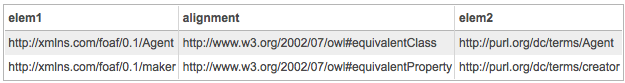
\includegraphics[width=1.0\linewidth]{equivalentCandR.png}
      \caption{Equivalent classes and properties between foaf and dcterms}
      \label{fig:eqCR}
    \end{figure}
    
 \item [Ontology Localization.] Labels in different languages are stored in the LOV endpoint for the ontology terms that provide such information. This annotations could be used when translating terms into different languages. This information could be extracted by querying the SPARQL endpoint\footnote{\url{http://goo.gl/JJCJ01}} as shown in Listing \ref{list:person} where all the labels defined for the terms that have at least one \emph{rdfs:label} containing strictly ``person":
		
    \begin{lstlisting}[float=htb,caption={SPARQL query asking all the labels defined for the terms containing person.},label=list:person, language=json]
    SELECT DISTINCT ?label2 ?element{
		?element rdfs:label ?label1 .
		?element rdfs:label ?label2 .
		FILTER (?label1 != ?label2 ).
		FILTER(REGEX(STR(?label1), "person", "i")).
	} ORDER BY ?element
	\end{lstlisting}
							
   An excerpt of the query result is shown in Figure \ref{fig:translations}. From that result, ``Persona''@es and ``Personne''@fr could be used as translations for the English term ``Person'' in Spanish and French respectively. 
   
   \begin{figure}[ht!b]
     \centering
     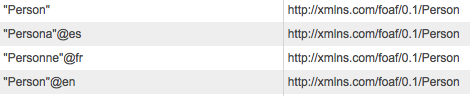
\includegraphics[width=.90\linewidth]{translations1.png}
     \caption{Translations example for foaf:Person}
     \label{fig:translations}
   \end{figure}
   
\end{description}

Figure \ref{fig:LOVandNeOn} shows the activities in which LOV can support within the overall Neon methodologies activity workflow.
\begin{figure}[h!tp]
\centering
  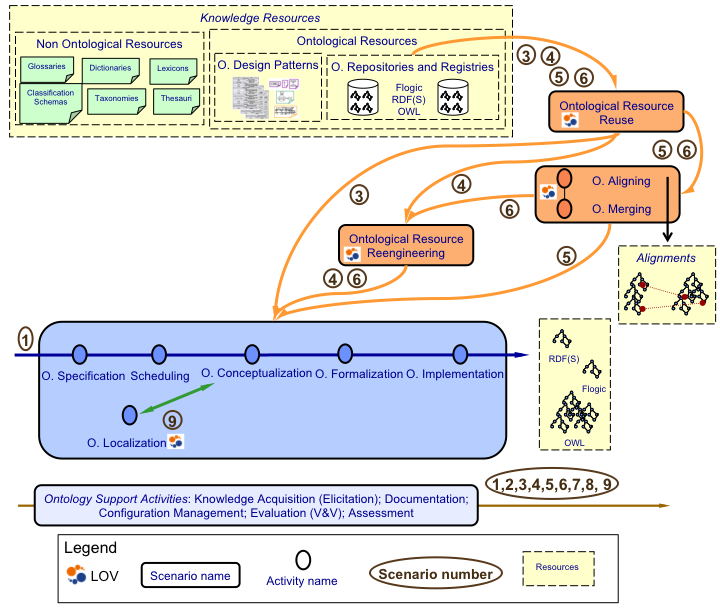
\includegraphics[width=.80\linewidth]{neonScenarios.png}
  \caption{Meeting points between LOV and the NeOn methodology, derived from \cite{MC10}.}
  \label{fig:LOVandNeOn}
\end{figure}

\section{LOV application and project ecosystem}
\label{sec:lovecosystem}
\py{ write the way to use the API, with a snapshot of some results}
LOV database as of today contains over 46,000 RDF vocabularies elements, with 28,000 properties and 18,000 classes, all accessible also via API\footnote{\url{http://lov.okfn.org/dataset/lov/apidoc/}}. For example, using the LOV Search API, an application can search for all classes with the term ``Catalog'' in any literal value by making the following call: \url{http://lov.okfn.org/dataset/lov/api/v2/search?q=Catalog&type=class}
 
\subsection{Derived tools and applications}

Maguire et al. \cite{ontomaton12} uses the LOV search API to implement OntoMaton\footnote{\url{https://github.com/ISA-tools/OntoMaton}}, a widget for bringing together ontology lookup and tagging within the collaborative environment provided by Google spreadsheets. 

YASGUI (Yet Another SPARQL Query GUI)\footnote{\url{http://yasgui.laurensrietveld.nl}}, a client-side JavaScript library that uses property, class and prefixes autocompletion using LOV API together with \url{http://prefix.cc} \cite{yasgui}.

Datalift\footnote{\url{http://datalift.org/en/node/24}} platform \cite{scharffe_2012}, a framework for ``lifting'' raw data into RDF, comes with a module to map data objects and properties to ontology classes and predicates available in the LOV catalogue. Data2Ontology module takes an input a ``raw RDF'', that is a dataset that has been converted directly from legacy format to triples. The goal is to help to publishers reusing existing ontologies for converting their dataset for easy discovery and interlinking. It consists of three main components assisting the publisher in selecting properties suitable for the dataset to be published. 
\begin{description}
\item[$\odot$~ \textbf{LOV component:}] This component is in charge to connect with the LOV catalogue to retrieve up-to-date ontologies using the LOV search API\footnote{\url{http://lov.okfn.org/dataset/lov/apidoc/\#lov2search}}.
\item[$\odot$~ \textbf{Matching Workflow:}] Data2Ontology offers to map the data to LOV by automatically proposing a list of best matches.

 \item[$\odot$~ \textbf{SPARQL Generator:}] This module receives as input the desired mappings and creates the SPARQL CONSTRUCT query needed to implement the mapping. The query can further be modified before the execution to generate a new dataset in the lifting process with Datalift.
 \end{description}

\subsection{Using LOV as a Research platform}
%\maria{ write input of your work on onto pitfalls using LOV dataset }. \\

LOV vocabularies have served as object of study in \cite{poveda2012landscape} where trends in ontology reuse techniques were analyzed in 2012. In addition, LOV dataset has been used in order to analyze the occurrence of good and bad practices in vocabularies as described in \cite{poveda2013detecting} in 2013.

Prefixes in LOV dataset is regularly mapped with namespaces in the prefix.cc service. In \cite{wasabi13}, the authors performs alignments of Qnames of vocabularies in both services, and provides different solutions to handle in case of clashes and disagreements on preferred namespaces. Both LOV and prefix.cc provide associations between prefixes and namespaces but following a different logic. The prefix.cc service supports polysemy and synonymy, and has a very loose control on its crowd-sourced information. In contrast, LOV has a much more strict policy forbidding polysemy and synonymy ensuring that each vocabulary in the LOV database is uniquely identified by a unique prefix identification allowing the usage of prefixes in various LOV publication URIs. This requirement leads sometimes to a situation where LOV uses prefixes different from the ones recommended by the vocabulary publishers.

LOV query log covering the period between 06/01/2012 and 16/04/2014 is used in \cite{butt2014} to build a benchmark suite for ontology search and ranking. The CBRBench\footnote{\url{https://zenodo.org/record/11121}} benchmark uses eight ranking models of resources in ontologies and compare the results with ontology engineers.

In \cite{janowicz2014five}, the authors rate vocabularies according to some criteria beyond the sameAs links but subClassOf and equivalentClass 'links' between vocabularies to foster interoperability, query federation, ease the interpretation of data, and so forth. %\ghis{ read this paper to add more content here}

Databugger\footnote{\url{https://github.com/AKSW/Databugger}} is a test-driven data debugging framework for the Web of Data. In \cite{databugger,rdfunit}, the authors provide an automatic test case instantiations for all available schemata registered with LOV. In this case, the vocabularies of LOV are used to encode semantics to domain specific knowledge to check the quality of data.

Giovanni et al. \cite{governatori2014} analyzes the current use of licenses in vocabularies on the Web based on LOV catalogue to further propose a framework to detect incompatibilities between datasets and vocabularies.


\section{Related work and Discussion}
\label{sec:related}

Reusing vocabularies requires searching for terms in existing specialized vocabulary catalogs or search engines on the web. While we refer the reader to~\cite{AquinJoWS12} for a systematic survey of ontology repositories, we list below some existing catalogs relevant to find vocabularies \cite{wasabi13}:
\begin{itemize}
 \item \textit{Catalogs of generic vocabularies/schemas} similar to the LOV catalog. Example of catalogs falling in this category are vocab.org\footnote{\url{http://vocab.org/}}, ontologi.es\footnote{\url{http://ontologi.es/}}, JoinUp Semantic Assets or the Open Metadata Registry.
 \item \textit{Catalogs of ontologies for a specific domain} such as biomedicine with the BioPortal \cite{bioportal11}, geospatial ontologies with SOCoP+OOR\footnote{\url{http://socop.oor.net/}}, Marine Metadata Interoperability and the SWEET \cite{sweet05} ontologies\footnote{\url{http://sweet.jpl.nasa.gov/2.1/}}. The SWEET ontologies include several thousand terms, spanning a broad extent of Earth system science and related concepts (such as data characteristics), with the search tool to aid finding science data resources. 
 \item \textit{Catalogs of ontology Design Patterns (ODP)} focused on reusable patterns in ontology engineering \cite{presutti08}. The submitted patterns are small pieces of vocabularies that can further be integrated or linked with others vocabularies. ODP is more targeted on  reusable successful solution to a recurrent modeling problem. However, it does not provide a search function for specific terms as it is the case with Swoogle or Watson.
 \item \textit{Search Engines of ontology terms}. Among ontology search engines, we can cite: Swoogle \cite{finin2005swoogle}, Watson \cite{d2007watson,Sabou07} and FalconS \cite{cheng2008falcons}. These search engines crawl for data schema from RDF document on the Web. They offer a filtering based on ontology type (Class, Property) and a ranking based on the popularity. They don't look for ontology relations nor check if the definition of the ontology is available (usually known as dereferenciation)
\end{itemize}


LOV focuses only on vocabularies (subpart of semantic documents of the web) submitted by any user, reviewed and validated by curators. In addition, LOV keeps track of different versions of the vocabularies in the server that can be retrieved for comparing the differences between along the time evolution.  In contrast, Swoogle is designed to automatically discover Semantic Web Documents (SWDs), indexes their metadata and answers queries about it. Thus, the result of a search query retrieved any semantic document. For example, a query of the term \textit{person} gives $16,438$ results while in LOV, only the term appears in $134$ vocabularies.
Watson works similarly to Swoogle, crawling and indexing semantic document at a small scale, explicitly distinguishing for each document (resource), concepts, properties and individuals if available. While in Swoogle  the ranking score is displayed, Watson shows the language of the resource and the size. Falcons is a keyword-based search system for concepts and objects on the Semantic Web, and is equipped with entity summarization for browsing. It is notable that Falcons limits the search only to ontologies and a recommendation feature is provided according to users' preferences. However, it does not provide any relationships between the related ontologies, nor any domain classification of the vocabularies.
Table \ref{tab:lovfeatures} lists some key features of LOV with respect to Swoogle, Watson and Falcons.
 \begin{table*}[!htb]
\centering{
\begin{tabular}{lllll}
\hline
 \textbf{Feature}	& Swoogle & Watson & Falcons & LOV 			 \\ \hline
Browsing ontologies	   & Yes & Yes & Yes & Yes \\
Scope & SWDs & SWDs & Concepts & ontologies \\
Metrics	& Ranking & Ranking & Ranking &  LOD popularity	 \\
Domain filtering & No & No & No & Yes \\
Comments and review 	& No & Yes & No & Only by curators	\\
Ranking	& Doc. based & Doc. based & Doc. based & Metric-based			\\
Web service access & Yes & Yes & Yes & Yes		\\
SPARQL endpoint	& No & No & No & Yes		\\
Read/Write	& Read & Read \& Write & Read &Read  	\\
Ontology directory & No & No & No &Yes \\
Application platform & No & No & No & Yes \\
Storage & Cache & - & - & Dump \& endpoint \\
Interaction with Contributors & No &  - & No & Yes \\

		\\ \hline

\end{tabular}
\caption{Comparison of LOV, with respect to Swoogle, Watson and Falcons; based on part of the framework defined in \cite{AquinJoWS12}.  }
\label{tab:lovfeatures}
}
\end{table*}

LOV search engine is to the best of our knowledge, the only purpose-built ontology search engine available on the Web with an up-to-date index.

\section{Conclusion and Future work}
\label{sec:conclusion}
\TODO{ add summary} \\
Next version v3 functionality coming soon :)

\section*{Acknowledgments}
This work has been partially supported by the French National Research Agency (ANR) within the Datalift Project, under grant number ANR-10-CORD-009 and the Spanish project BabelData (TIN2010-17550) and Fujitsu Laboratories. The Linked Open Vocabularies initiative is graciously hosted by the Open Knowledge Foundation.Thanks to all the members of the LOV community in Google+\footnote{\url{https://plus.google.com/communities/108509791366293651606}}, all the editors and publishers of vocabularies who trust in the LOV catalogue. 


\bibliographystyle{plain}
\bibliography{lov}
\end{document}
